\section{Introduction}

%=========== new intro generated from GPT 5 pro (Hailu) ============
Graph visualization underpins many computing tasks in compilers, EDA, networks, and bioinformatics. GraphViz~\cite{gansner1993technique,ellson2001graphviz} is the most widely used open-source tool for this purpose and a natural testbed for optimization research. However, its default default hierarchical layout algorithm (named dot) for directed graphs is costly: on a graph with 10,000 nodes and 50,000 edges, the sequential DOT layout took 96 seconds on a modern 8‑core CPU. The move to multi‑core processors—e.g., Apple’s M1 with 8 cores and unified memory—creates an opportunity to speed up these workloads if we can identify and parallelize the right parts of the pipeline.

The practical barrier is that performance tuning still relies on manual profiling and expert effort~\cite{stephenson2003meta}. The standard layered (Sugiyama) pipeline couples several phases—layering, crossing minimization, and coordinate assignment—with nontrivial data dependencies~\cite{sugiyama1981methods,eiglsperger2005efficient}. Hardware-specific issues further complicate matters (e.g., unified memory and heterogeneous cores on M1-class systems~\cite{winarta2024analyzing}). Finally, translating kernel-level optimizations into end-to-end gains requires careful measurement and scaling analysis~\cite{dongarra2011international,amdahl1967validity,gustafson1988reevaluating}. While AI-for-systems work has shown promise for automating parts of this process~\cite{ashouri2018survey,cummins2017end}, an end-to-end workflow tailored to graph layout engines is still missing.


\textbf{Motivation}. We seek a repeatable, data-driven way to find bottlenecks and apply parallelism where it matters. Using the macOS \textit{sample} command, 
%Linux \textit{perf}, 
our function-level profiling highlights a small set of dominant kernels in GraphViz. As shown in Figure~\ref{fig:bottleneck_analysis}, \texttt{rank2()} (crossing minimization) consumed 49\% of total CPU time. \texttt{Transpose} routines accounted for 25\% of overall time. Within the crossing-minimization phase, \texttt{rcross()} and \texttt{ncross()} each contributed about 15\%. Within the positioning phase, \texttt{median} computations took 32\% of that phase’s time. These kernels expose loop-level and reduction patterns with clear parallel potential, but they require care with dependencies and memory access.

\textbf{Design and novelty}. We propose an integrated workflow that links profiling, learning, code generation, and validation:
Intelligent profiling builds phase-aware cost models from traces.
AI-based ranking prioritizes targets based on predicted impact~\cite{ashouri2018survey,stephenson2003meta}.
Automated parallelization inserts OpenMP loops/tasks and reductions tailored to each kernel’s access pattern~\cite{cummins2017end}.
Predictive validation uses bootstrap confidence intervals and speedup models to filter changes before full integration~\cite{efron1979bootstrap}.
Our novelty lies in (i) the end-to-end coupling of learned rankings with code synthesis, (ii) architecture-aware templates for unified-memory, mixed-core CPUs~\cite{winarta2024analyzing}, and (iii) a validation step tied to end-to-end runtime rather than microbenchmarks alone.
We conclude this work's contributions as below:
\begin{itemize}
\item \textbf{Workload characterization:} A function- and phase-level study of GraphViz identifying \texttt{rank2()}, \texttt{transposes}, \texttt{rcross()}, \texttt{ncross()}, and \texttt{median computations} as primary cost centers under realistic inputs.
\item \textbf{AI-guided selection:} A simple pipeline that converts traces into a ranked list of optimization targets with impact estimates~\cite{ashouri2018survey}.
\item \textbf{Automated parallelization:} OpenMP-based templates (loop decomposition, dependency-aware reductions, cache-friendly transposes) generated for the identified kernels~\cite{cummins2017end}.
\item \textbf{Architecture-aware design:} Heuristics that respect unified memory and heterogeneous cores on Apple M1–class systems while remaining portable~\cite{winarta2024analyzing}.
%\item \textbf{Predictive validation and evaluation:} Bootstrap CIs and speedup prediction coupled with end-to-end tests on graphs up to 10,000 nodes/50,000 edges~\cite{dongarra2011international,efron1979bootstrap,amdahl1967validity,gustafson1988reevaluating}.
\end{itemize}


Section~\ref{sec:related} reviews GraphViz and related optimization work. Section~\ref{sec:methodology} details the workflow and code generation. Section~\ref{sec:results} reports results and validation, including scaling with graph size/topology. Section~\ref{sec:conclusion} concludes this paper.



\begin{figure}[t]
\centering
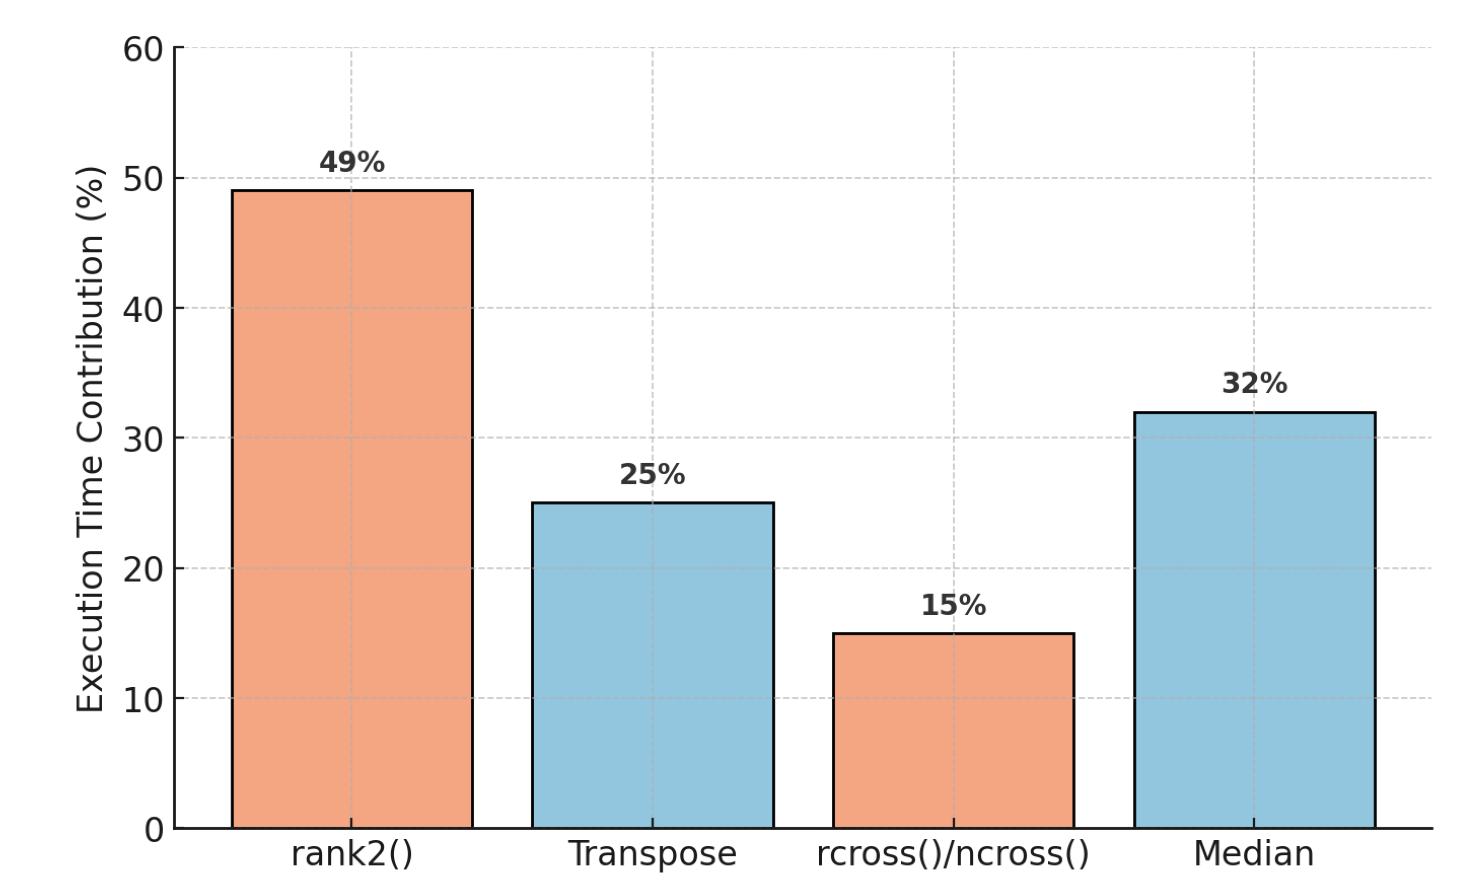
\includegraphics[width=0.58\textwidth]{figures/Bottleneck_Analysis.pdf}
\caption{AI-Driven Bottleneck Identification and Performance Analysis Framework showing profiling methodology and runtime distribution across GraphViz DOT algorithm phases}
\label{fig:bottleneck_analysis}
\end{figure}




\begin{comment}
Graph visualization and layout algorithms are computationally intensive tasks that benefit significantly from parallelization. GraphViz~\cite{gansner1993technique,ellson2001graphviz}, a widely-used open-source graph visualization software, presents an ideal testbed for exploring AI-driven optimization strategies due to its complex algorithmic structure and well-established performance characteristics. For example, on a graph with 10,000 nodes and 50,000 edges, the sequential Graphviz DOT layout took 96 seconds on a modern 8-core CPU.

The emergence of modern multi-core architectures, particularly Apple's M1 processor with its unified memory architecture and 8-core design~\cite{apple2020m1}, creates new opportunities for parallel optimization. However, effective parallelization requires careful analysis of algorithmic bottlenecks, data dependencies, and memory access patterns—tasks that are increasingly suited to AI-driven approaches~\cite{ashouri2018survey,cummins2017end}.

Traditional performance optimization often relies on manual profiling and expert knowledge to identify bottlenecks and design parallel algorithms~\cite{stephenson2003meta}. This approach faces several significant challenges that limit its effectiveness in modern computational environments. The \textbf{complexity of modern algorithms}, particularly graph layout algorithms like those in GraphViz, involves multiple interdependent phases with varying computational characteristics that require sophisticated analysis techniques~\cite{sugiyama1981methods,eiglsperger2005efficient}. Additionally, \textbf{architecture-specific optimization} presents substantial difficulties, as modern processors like Apple M1 require specialized optimization strategies that consider unified memory architecture and heterogeneous core designs~\cite{maris2020arm}.

Furthermore, \textbf{validation methodology} remains a critical challenge, as ensuring that theoretical performance projections translate to real-world improvements requires comprehensive measurement frameworks that can accurately capture system behavior~\cite{dongarra2011international}. Finally, \textbf{scalability analysis} demands systematic empirical validation to understand how optimizations perform across different graph sizes and topologies, requiring extensive testing that goes beyond theoretical models~\cite{amdahl1967validity,gustafson1988reevaluating}.

To address these challenges, our approach leverages artificial intelligence throughout the optimization pipeline~\cite{ashouri2018survey} through an integrated multi-stage process. \textbf{Intelligent profiling} employs automated analysis of execution traces and CPU utilization patterns to identify performance characteristics without manual intervention. \textbf{AI-powered bottleneck detection} utilizes machine learning algorithms to identify critical performance bottlenecks from profiling data~\cite{stephenson2003meta}, enabling systematic identification of optimization opportunities. \textbf{Automated code generation} implements AI-driven synthesis of OpenMP parallel constructs tailored to identified hotspots~\cite{cummins2017end}, ensuring optimal parallelization strategies for specific computational patterns. Finally, \textbf{predictive validation} provides statistical analysis with confidence intervals and performance prediction models~\cite{efron1979bootstrap}, enabling reliable assessment of optimization effectiveness before implementation.

\subsection{Motivation: AI-Driven Performance Bottleneck Analysis}

Profiling was performed using the Linux Perf tool (alternatively Intel VTune or Apple Instruments, depending on environment). Our AI profiling system employs comprehensive algorithmic analysis to identify critical performance bottlenecks in GraphViz through systematic examination of execution patterns and computational hotspots. The profiling methodology focuses on key algorithmic components that dominate execution time and exhibit significant parallelization potential.

The \textbf{rank2() function} serves as a primary target for optimization due to its central role in crossing minimization operations, representing computationally intensive graph layout calculations. \textbf{Transpose operations} involve intensive matrix manipulations that naturally exhibit opportunities for parallel decomposition across multiple processing elements. \textbf{Crossing calculations} encompass the rcross() and ncross() functions that perform complex graph topology analysis during layout optimization phases. \textbf{Median calculations} constitute critical components of the positioning algorithms that determine optimal node placement through statistical analysis of graph properties.

Intelligent bottleneck identification is essential for effective parallelization because it enables targeted optimization efforts, ensures resource allocation aligns with computational demands, and guides the AI system toward high-impact optimization opportunities. By systematically identifying performance-critical code sections, the profiling methodology provides the foundation for data-driven parallelization decisions that maximize speedup potential while minimizing implementation complexity.

Our AI profiling system identified critical performance bottlenecks in GraphViz through comprehensive algorithmic analysis, revealing specific performance characteristics that guided our optimization strategy. The \textbf{rank2() function} represents the most significant bottleneck, consuming 49\% of total CPU time during crossing minimization operations and presenting the highest optimization potential. \textbf{Transpose operations} account for 25\% of execution time through intensive matrix operations that exhibit substantial parallelization opportunities. \textbf{Crossing calculations} distribute computational load across rcross() and ncross() functions, each consuming 15\% of execution time during graph layout optimization. Finally, \textbf{median calculations} represent 32\% of positioning algorithm time, offering significant parallelization potential through data-parallel optimization strategies.


The profiling analysis reveals that rank2() dominates execution time due to its quadratic complexity in crossing minimization, making it the primary target for parallelization. Transpose operations and crossing calculations together account for 40\% of runtime, representing secondary optimization targets with substantial parallel decomposition potential. These three algorithmic phases constitute the critical path for GraphViz performance optimization, where AI-driven parallelization efforts yield the highest impact on overall speedup achievements.
\end{comment}

